\section{Object Database}

Generally, particular object shape and color usage bring a certain bias to the learned grasp model. Therefore, the object database should be as diverse as possible to encourage the model to perform well on novel objects. Indeed, the generalization of all different shapes and colors of the objects is our primary concern. Since we measure the success rate of an RL agent on the test set, a model that overfits the training dataset would perform poorly on the test set.

We use the random object database(\ref{fig:randomobj}) from pybullet-data \footnote{\url{https://bit.ly/3ijyCJM}} and the wooden-block datasets(\ref{fig:woodenobj}) from Breyer et al. for our experiments. We trained only on the random object database. Wooden blocks dataset was only used to test the robustness of the trained model.

Unlike, Quillen et al. and Breyer et al. which divided their dataset only into test and training, we used a validation set in addition to them.  We believe the inclusion of the validation set contributes to the generalization of the trained model. In total, test and validation sets have 150 objects each, and training sets consist of 700 objects.

\begin{figure}

    \begin{subfigure}{1.0\textwidth}
      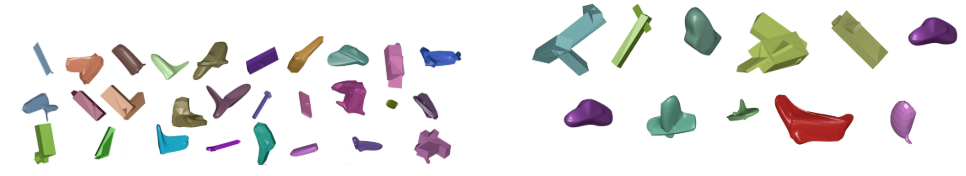
\includegraphics[width=\linewidth]{figures/random_objects}
      \caption{Random object dataset} \label{fig:randomobj}
    \end{subfigure}%
    \hspace*{\fill}   % maximize separation between the subfigures
    \newline
    \begin{subfigure}{1.0\textwidth}
      \centering
      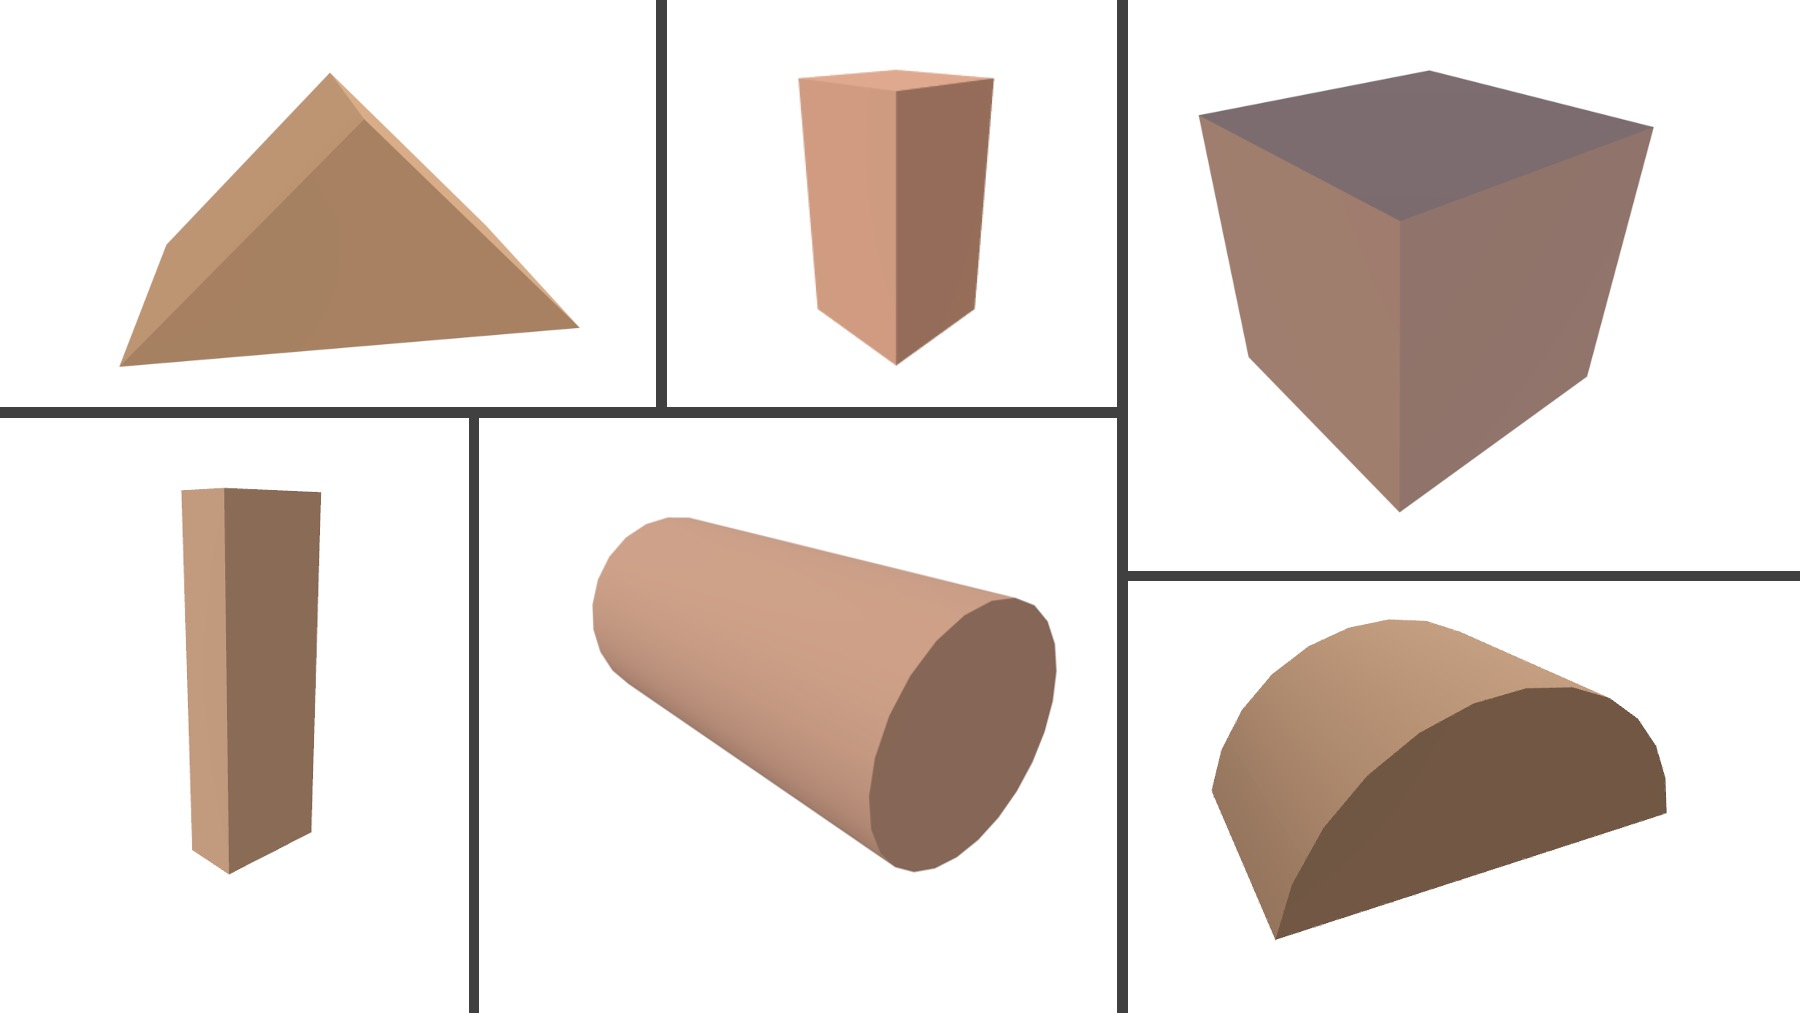
\includegraphics[width=0.3\linewidth]{figures/wooden_blocks}
      \caption{Wooden block dataset from Breyer et al. \cite{Breyer2018}} \label{fig:woodenobj}
    \end{subfigure}%
    \hspace*{\fill}   % maximize separation between the subfigures
\caption{ Different object datasets used in our work \label{fig:objdatasets}}
\end{figure}